% !TEX program = pdflatex
%
% 4-page course-submission version of the report.
% The long (16-page) version with full discussion, failure-mode
% post-mortem, and extended limitations lives in main.tex.
%
\documentclass[11pt]{article}

\usepackage[margin=0.8in]{geometry}
\usepackage[utf8]{inputenc}
\usepackage[T1]{fontenc}
\usepackage{lmodern}
\usepackage{microtype}

\usepackage{amsmath}
\usepackage{amssymb}
\usepackage{booktabs}
\usepackage{graphicx}
\usepackage{caption}
\usepackage{xcolor}
\usepackage[hidelinks]{hyperref}

\setlength{\parskip}{2pt}
\setlength{\parindent}{1em}

\title{\vspace{-3em}Multi-turn GRPO with Real Tool Execution for a Research Agent on HotpotQA}
\author{Yue Wu}
\date{\vspace{-0.5em}\today}

\begin{document}
\maketitle
\vspace{-1.5em}

\begin{abstract}
\noindent
We build a small tool-using research agent on HotpotQA:
Qwen2.5-0.5B-Instruct with LoRA, fine-tuned by SFT on synthetic
interaction traces, then refined by multi-turn GRPO whose rollouts
execute the real BM25 retrieval tool at every step rather than a
model-generated (``virtual'') trace. On 100 HotpotQA validation
questions, the full pipeline lifts exact-match from 26\% (best
zero-shot stopping heuristic) to 44\%. Decomposing this gap, we
find that the bulk comes from a single inference-time change:
aligning the rollout step budget with the SFT trajectory length
lifts the SFT policy alone to 42--44\%, while multi-turn GRPO on
top produces no detectable lift at our evaluation scale. We trace
the null result to tied reward groups --- 159 of 200 training
epochs had identical rewards across the $G{=}4$ rollouts, so the
effective update budget was $\sim$41, not 200 --- and argue that
the next bottleneck is reward design (a term with continuous
intra-group variance on all-wrong groups), not more or longer
training.
\end{abstract}

\vspace{-0.5em}

% ==========================================================
\section{Introduction}
\label{sec:intro}

A \emph{research agent} is a language model that answers a user's
question by issuing real tool calls --- typically a search API
--- and reasoning over the retrieved content over several
rounds, as exemplified at the product level by systems like
Perplexity and OpenAI's Deep Research \cite{deep-research}. At
the research level, ReAct \cite{react} established the
interleaved reason-and-act pattern and Toolformer
\cite{toolformer} showed that a language model can learn
\emph{when} to invoke an external API by self-supervision.
Separately, policy-gradient post-training of language models has
grown out of PPO-based RLHF \cite{rlhf-instructgpt} into the
GRPO procedure popularised by DeepSeek-R1 \cite{deepseek-r1},
which removes the critic network and normalises rewards within a
group of rollouts. Most RL-for-LLM recipes, including R1, train
on self-generated \emph{virtual} rollouts where the model emits
both the action and the fake tool output. This creates a
distribution mismatch: at inference a real retrieval index
produces observations a small policy would never hallucinate. We
study what happens if we close that gap --- running GRPO rollouts
that execute the real BM25 tool at every step --- on a small
0.5B-parameter open policy.

Our testbed is HotpotQA distractor \cite{hotpotqa}, a two-hop
multi-document QA benchmark. We compare three regimes: (i)~a
supervised fine-tuned (SFT) policy evaluated under five zero-shot
stopping heuristics (fixed step budget, confidence threshold,
run-to-max); (ii)~the same SFT policy run with the full trajectory
length it was trained on; (iii)~multi-turn GRPO on top of the SFT
policy, with real tool execution.

The headline gap from the best zero-shot baseline (26\% EM) to
multi-turn GRPO (44\%) is 18 points, but this is misleading on
inspection: 16 of the 18 points come from a single inference-time
change (running the SFT policy for its full 5-step trajectory),
and GRPO on top contributes no measurable lift within our
evaluation noise. We then diagnose why (\S\ref{sec:discussion}).

\vspace{-0.3em}

% ==========================================================
\section{Method}
\label{sec:method}

\paragraph{Task and environment.}
The agent receives a natural-language question and must emit a
short free-form answer $\hat a$, scored by the HotpotQA official
normalisation (lower-case, strip punctuation + articles,
exact-match-or-substring). The retrieval environment is a
deterministic BM25 index over 66{,}576 Wikipedia paragraphs from
the HotpotQA validation split. Two tool actions are exposed:
\texttt{search(query)} returning the top-2 documents with $\approx$300-
character snippets, and \texttt{read(doc\_id)} returning the full
document text clipped to 300 characters. The same index is used
by all three regimes so every row in Table~\ref{tab:main} sees an
identical environment.

\paragraph{Policy.}
Qwen2.5-0.5B-Instruct \cite{qwen25} with a LoRA adapter on
attention \emph{and} MLP projections
($\{q,k,v,o,\mathrm{gate},\mathrm{up},\mathrm{down}\}_\texttt{proj}$),
rank $r{=}16$, $\alpha{=}32$, dropout 0.05. At each step the
policy emits one JSON object with keys
\texttt{\{thought, action, query\,|\,document\,|\,answer, confidence\}}.

\paragraph{Supervised fine-tuning.}
We generate 6{,}000 five-step training traces from HotpotQA
supporting facts. For each training example we build a per-example
BM25 mini-index over its 10 context paragraphs, issue a real
\texttt{search} with a query built from the question and the
supporting title, and keep the trace iff BM25 surfaces the gold
document; the resulting trajectory is
\texttt{search}$\to$\texttt{read}$\to$\texttt{search}$\to$\texttt{read}$\to$\texttt{answer}.
Loss is computed only on the policy's own JSON actions: tokens
that fall inside injected \texttt{Observation:} lines (identified
via the tokenizer's \texttt{offset\_mapping}) are masked with
\texttt{IGNORE\_INDEX}. This observation-masked loss is the
single biggest engineering lever in the SFT stage; before it was
in place the model had never seen real retrieval output at
training time. Training runs for 5 epochs with AdamW at
$2{\times}10^{-4}$ on a T4; the best-eval-loss checkpoint is used.

\paragraph{Multi-turn GRPO with real tool execution.}
For each training question we sample $G{=}4$ interactive rollouts.
Each rollout is a sequence of \emph{real} tool dispatches:
\texttt{model.generate} emits a JSON action, we parse the
\texttt{action} field, execute the corresponding BM25 call, and
splice the real observation into the prompt before the next
generation step, up to $\mathrm{max\_steps}{=}5$. The scalar reward
combines correctness ($+1.0$ on exact-match), a format score (up
to $+0.10$ for valid JSON with required keys and an
\texttt{answer} action), and efficiency terms that penalise step
count and pairs of consecutive steps whose confidence values have
low Jensen-Shannon divergence. The within-group advantage is the
$z$-score
$A_i = (R_i - \bar R)/(\sigma_R + \varepsilon)$, and the policy-
gradient loss on rollout $i$ is
$\mathcal{L}_i = -A_i \sum_{t\in\mathcal{G}(\tau_i)} \log \pi_\theta(\tau_{i,t}|\tau_{i,<t})$
with $\mathcal{G}(\tau_i)$ the set of policy-generated token
positions (observation tokens masked out via
\texttt{offset\_mapping}, as in SFT).

\paragraph{Engineering choices.}
Three details matter at our scale. \emph{(a)~Rollout temperature
0.5} (not the DeepSeek-R1 default of $\approx$0.9): at 0.9 the
0.5B policy loses JSON format on the first step and every rollout
terminates at step one with an empty answer, killing training.
\emph{(b)~Rollouts run in \texttt{model.eval()}} so LoRA dropout
is disabled during generation;
\texttt{@torch.no\_grad()} alone is \emph{not} sufficient, because
it disables gradient tracking but not dropout. \emph{(c)~Per-episode
backward}: we pre-scale each rollout's loss by $1/(G\cdot|\text{batch}|)$,
call \texttt{loss.backward()} immediately, free the activation
graph, and only run \texttt{optimizer.step()} after all
$G{=}4$ rollouts. Peak VRAM is one trajectory's activations
($\approx$6--8~GB at 1{,}500 tokens bf16) rather than
$G{\cdot}|\text{batch}|$ trajectories held simultaneously. This
memory budget is also the reason we \emph{omit} a KL-to-reference
term: a frozen-reference forward would double peak activation
memory and push the T4 to OOM. The small LoRA adapter
(${\sim}2$M trainable of ${\sim}500$M total) acts as an implicit
drift regulariser, and 200 GRPO steps is short enough that
long-horizon KL drift is not the binding constraint.

We pre-filter candidate training questions with a learnable-zone
check: $K{=}3$ eval-mode rollouts per question, keep groups where
$n^{\mathrm{corr}}_q \in \{0,1,2\}$ (excluding only ``all correct''
groups; all-wrong groups with non-degenerate format variance still
produce usable advantages). From 200 candidates the filter keeps
${>}180$.

% ==========================================================
\section{Experiments}
\label{sec:experiments}

\paragraph{Setup.}
All evaluation is on the first 100 questions of HotpotQA distractor
validation split with near-greedy decoding ($T{=}0.1$,
$\mathrm{max\_steps}{=}5$) against the 66{,}576-document BM25 index.
Zero-shot baselines share the Week-1 SFT adapter with no further
training and differ only in the inference-time stopping rule:
\textbf{FixedStep($N$)} forces exactly $N$ steps and treats the
last as the answer; \textbf{Confidence($\tau$)} stops at the first
step whose \texttt{confidence} exceeds $\tau$;
\textbf{NeverStop(max=6)} ignores any emitted \texttt{answer}
action and runs for six steps.

\begin{table}[h]
\small
\centering
\caption{100 HotpotQA validation questions, same BM25 index across
all rows. The first five rows share the SFT adapter and differ
only in inference-time stopping. The last two rows run the full
5-step trajectory.}
\label{tab:main}
\begin{tabular}{lcc}
\toprule
Method & EM (\%) & Avg.\ steps \\
\midrule
FixedStep($N{=}2$)         & 6.0  & 2.00 \\
FixedStep($N{=}3$)         & 16.0 & 2.50 \\
Confidence($\tau{=}0.75$)  & 20.0 & 2.88 \\
Confidence($\tau{=}0.85$)  & 26.0 & 3.20 \\
NeverStop($\max{=}6$)      & 21.0 & 3.57 \\
\midrule
\textbf{SFT-only @ $\max_{\text{steps}}{=}5$}$^{\dagger}$ & \textbf{42.0\,/\,44.0} & \textbf{5.00} \\
\textbf{Multi-turn GRPO (ours)}                          & \textbf{44.0}          & \textbf{4.99} \\
\bottomrule
\end{tabular}
\vspace{0.2em}
{\footnotesize
\\ $^{\dagger}$~Two independent evaluations of the same SFT adapter
on the same 100 questions at $T{=}0.1$. The 2-pp spread is the
within-run sampling variance at $n{=}100$; the GRPO value sits
inside that spread.}
\end{table}

\begin{figure}[h]
\centering
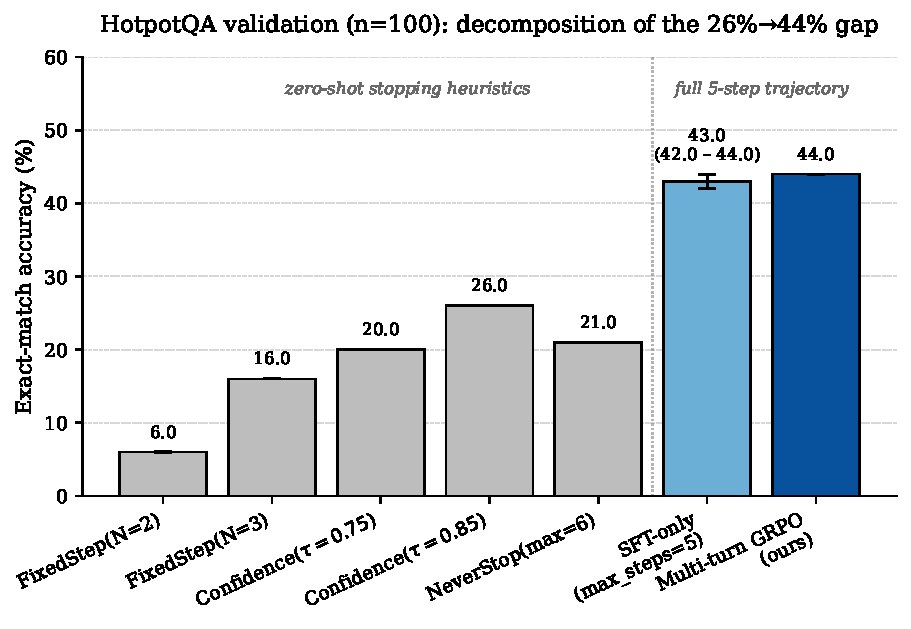
\includegraphics[width=0.8\linewidth]{figures/fig1_main.pdf}
\vspace{-0.6em}
\caption{Exact-match accuracy across the zero-shot baselines (grey)
and the two 5-step configurations: SFT-only (light blue) and GRPO
(dark blue). Error bar on SFT-only is the two-run spread
(42.0--44.0); GRPO sits inside it.}
\label{fig:main}
\end{figure}

\vspace{-0.5em}

\paragraph{Main result.}
Table~\ref{tab:main} shows the $+18$-point gap from the best
zero-shot baseline (26\% EM) to multi-turn GRPO (44\%) decomposes
into two very different components. First, the zero-shot
baselines all cap the rollout at 2--6 steps through various
stopping heuristics, and EM rises monotonically with trajectory
length up to 26\%. When we simply remove every stopping heuristic
and let the SFT policy run for the full five steps it was trained
on, EM jumps to 42--44\% --- a $+16$-point move with \emph{no}
additional parameter update. Second, multi-turn GRPO at matched
inference settings scores 44.0\% at the same average trajectory
length (4.99 steps); two independent SFT-only evaluations on the
same 100 questions gave 42.0 and 44.0, bracketing the GRPO number,
so the GRPO lift over the matched baseline is $\leq$2~pp and
within one standard error at $n{=}100$ (Wald SE $\approx$4.9~pp
at $p{=}0.43$). We cannot claim that multi-turn GRPO improved EM
over SFT at the matched trajectory length from this evaluation.

\paragraph{Training dynamics.}
Of the 200 GRPO update steps, only 41 (20.5\%) produced a
non-zero training loss; the remaining 159 had tied rewards
across all $G{=}4$ rollouts and were skipped by the
$|A_i|<10^{-8}$ guard. The dominant tied configuration is
\emph{all four rollouts wrong with identical format score}: the
format reward saturates at $+0.10$ as soon as the policy emits
valid JSON with the required keys, so a group of all-wrong
rollouts is tied on every component. Validation EM across the 10
checkpoints ranges over $[0.35, 0.50]$ on 20-question subsamples
with $\approx$11-pp standard error and does not show a monotone
upward trend.

% ==========================================================
\section{Discussion}
\label{sec:discussion}

The null result of GRPO over SFT at matched inference is mostly
explained by the effective-updates analysis in the last
paragraph: 159/200 tied groups means the effective learning rate
is $\sim$5$\times$ smaller than it looks on paper, and at a LoRA
adapter with $\sim$2~M trainable parameters and
$\eta{=}5{\times}10^{-6}$, 41 effective updates is not enough to
move the policy in EM-detectable directions. It is also true that
the SFT-only policy at $\mathrm{max\_steps}{=}5$ scores 42--44\% ---
close to the retrieval-bottlenecked ceiling for a 0.5B model on
this task --- so even a well-calibrated GRPO run would have
limited headroom.

The key mechanism is the saturated format reward. On all-wrong
correctness groups, GRPO's within-group advantage is driven
entirely by format and efficiency variance, and our current
format reward is binary-on-two-keys with a small final kicker; it
saturates at 0.10 for essentially every well-formed rollout.
Continuous-variance alternatives (token-level JSON-validity
score, query-novelty score based on lexical overlap with previous
queries, document-overlap score across retrieved docs) would give
a usable gradient on the 80\% of training groups that are
currently tied. We view this as the tightest concrete next step
for making real-tool GRPO pay at sub-1B scale, above more-
compute or KL-stabilisation interventions.

\paragraph{Limitations.}
$n{=}100$ cannot resolve the $\leq$2-pp gap between SFT-only and
GRPO; a 500-question paired evaluation was prepared but not run
because Kaggle CPU time exceeded the 12~h kernel cap. The
omission of the KL-to-reference term is memory-driven (a
frozen-reference forward doubles peak activation memory on T4).
Results at 0.5B are unlikely to transfer linearly to 7B+ scale,
where the format-saturation mechanism changes. Full failure-mode
post-mortem and tuning journey are in the long-form report and
\texttt{TUNING\_JOURNEY.md}.

% ==========================================================
\section{Conclusion}
\label{sec:conclusion}

For a small SFT'd tool-using policy on HotpotQA, the dominant
lever from 26\% to 44\% EM is matching the inference trajectory
length to the SFT trajectory length (16 of 18 points), not the
reinforcement-learning step. Multi-turn GRPO with real tool
execution produces no measurable lift at $n{=}100$; the binding
constraint is reward design --- a saturating format term leaves
80\% of updates with tied advantages, and a continuous
intra-group-variance term is the most likely next intervention.

% ==========================================================
\bibliographystyle{plain}
\bibliography{refs}

% ==========================================================
% Appendix (does not count against the 4-page main-body budget)
% ==========================================================
\appendix

\section{Zero-shot baseline stop-reason breakdown}
\label{app:stop-reasons}

Table~\ref{tab:stop-reasons} reports \emph{why} each zero-shot
baseline's rollouts terminated on the 100 HotpotQA validation
questions. Three termination modes are possible: \texttt{answer}
means the policy emitted an \texttt{action:"answer"} step within
the step budget; \texttt{parse\_error} means the generation was
not a parseable JSON object with the required keys;
\texttt{policy} means the rollout hit the step-budget cap without
a valid \texttt{answer} action, in which case the last step's
text is taken as the predicted answer.

\begin{table}[h]
\small
\centering
\caption{Stop-reason counts (out of 100) for each Week 2
baseline. Compare to EM in Table~\ref{tab:main}.}
\label{tab:stop-reasons}
\begin{tabular}{lrrr}
\toprule
Method & \texttt{answer} & \texttt{parse\_error} & \texttt{policy} \\
\midrule
FixedStep($N{=}2$)         & 0  & 0   & 100 \\
FixedStep($N{=}3$)         & 0  & 50  & 50  \\
Confidence($\tau{=}0.75$)  & 7  & 48  & 45  \\
Confidence($\tau{=}0.85$)  & 12 & 44  & 44  \\
NeverStop($\max{=}6$)      & 53 & 47  & 0   \\
\bottomrule
\end{tabular}
\end{table}

Two things stand out. First, at $\mathrm{max\_steps}\leq 3$ the
policy essentially never emits a clean \texttt{answer} action ---
FixedStep($N{=}3$) has a 0\% answer rate, and even
Confidence($\tau{=}0.85$) only reaches 12\%. This is the
structural reason the best zero-shot baseline plateaus at 26\%
EM: most rollouts either parse-error or run out of steps. Second,
NeverStop pushes the answer rate up to 53\% by simply letting the
policy run further, and the SFT-only row of Table~\ref{tab:main}
(42--44\%) is the limiting case where the step budget matches the
SFT trajectory length exactly. The 16-point step-budget component
of our decomposition is visible directly in the monotone rise of
the \texttt{answer} column.

\section{GRPO training dynamics}
\label{app:training-dynamics}

\begin{figure}[h]
\centering
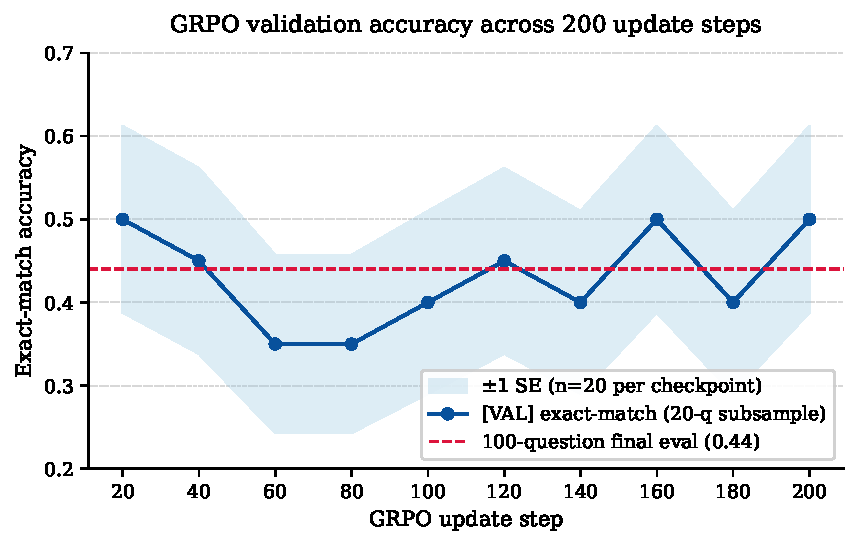
\includegraphics[width=0.8\linewidth]{figures/fig2_val.pdf}
\caption{GRPO validation exact-match across 200 training steps.
Each point is a freshly sampled 20-question subset of the HotpotQA
validation split; the $\pm 1$-SE band reflects the binomial
variance at $n{=}20$ only. The dashed line is the 100-question
final eval (0.44). The curve stays within $[0.35, 0.50]$ and does
not show a monotone improvement --- expected behaviour for a run
with only $\sim$41 effective gradient updates (see main-body §3).}
\label{fig:val_curve}
\end{figure}

Of the 200 GRPO update steps, exactly 41 (20.5\%) produced
non-zero training loss; the remaining 159 had identical rewards
across the $G{=}4$ rollouts and were skipped by the
$|A_i|<10^{-8}$ guard in \texttt{grpo\_train\_step}. Training
epoch time was $\approx$50--60~s on a T4, making the full run
$\approx$3~h including the learnable-zone filter and periodic
validation. Decomposing the tied-reward configuration, essentially
all tied groups came from \emph{all four rollouts wrong with
identical format score}; this is the pathology the main-body
\S4 prescription (continuous-variance format reward) is designed
to address.

\section{Failure modes encountered during tuning}
\label{app:failure-modes}

The final GRPO configuration reported in the main body is the
product of three debugging iterations, each triggered by a
specific empirical symptom. The full post-mortem, including
commit hashes and reproduction steps, is in the accompanying
\texttt{TUNING\_JOURNEY.md}; we summarise them briefly here
because they are collectively a small-but-general lesson about
multi-turn LM-RL at sub-1B scale.

\paragraph{(i) Rollout temperature.}
A first version used the DeepSeek-R1-style default $T{=}0.9$ for
rollout generation inside GRPO. On the 0.5B policy this is large
enough that the per-step JSON parse fails on step one, the
parse-failure branch terminates the rollout at step one with an
empty \texttt{answer}, and every group is tied at zero correctness
and identical format. The zone histogram reported \emph{zero}
learnable groups over 1{,}000 candidate questions. Fix: $T{=}0.5$,
threaded through \texttt{filter\_learnable\_questions} and
\texttt{grpo\_train\_step} as an explicit parameter rather than a
hardcoded default inside the leaf function.

\paragraph{(ii) Step budget matching SFT trajectory length.}
A second version used $\mathrm{max\_steps}{=}3$ for rollouts.
Rollouts reliably emit
\texttt{search}$\to$\texttt{read}$\to$\texttt{search} and end
\emph{before} the policy ever gets to \texttt{read}$\to$\texttt{answer}
for the second hop, since the SFT traces are 5 steps long. Every
rollout scored zero correctness regardless of retrieval quality.
Fix: $\mathrm{max\_steps}{=}5$, matching the SFT trajectory length.
This observation is the direct inspiration for the main-body
step-budget decomposition.

\paragraph{(iii) Eval mode during rollout.}
A third version called \texttt{collect\_episodes\_batched}
(decorated with \texttt{@torch.no\_grad()}) while the model was
in \texttt{train} mode. \texttt{no\_grad} disables gradient
tracking but \emph{not} dropout; the 0.05 LoRA dropout was still
active during generation, and the first-step JSON parse failed
often enough to reproduce the step-one-termination pathology from
(i). Symptom: \texttt{steps=1.0, acc=0.00, loss=0.0000} on every
training epoch, while the periodic \texttt{[VAL]} check (which
explicitly calls \texttt{model.eval()}) reported $\sim$35\%.
Fix: \texttt{model.eval()} immediately before the rollout,
\texttt{model.train()} immediately after, on a per-question
basis.

A common thread runs through all three: each was a hyperparameter
or code-path default that was correct for a \emph{larger} base
policy or a \emph{non-interactive} training loop, and silently
wrong for our setup.

\end{document}
